
%%%%%%%%%%%
%remove tag+probe ref
%%%%%%%%%%%


\section{Top Background Estimation}
\label{sec:topbkg}


The MET templates method is used to estimate the contribution of SM \Z production
 to the signal region due to the fake MET tail. However,
it does not account for the \ttbar background in which the dileptons happen to lie
 in the \Z mass window, which is accompanied by genuine MET. 
To estimate this contribution we use an opposite-flavor subtraction
technique which takes advantage of the fact that the \ttbar yield in the 
opposite-flavor final state ($e\mu$) is the same as in the same-flavor final state
($ee+\mu\mu$), modulo differences in efficiency in the $e$ vs. $\mu$ selection.
 Hence the \ttbar yield in the same-flavor final state can be estimated
using the corresponding yield in the opposite-flavor final state. 
It is important to note that other backgrounds for which the lepton flavors are
uncorrelated (for example $WW$ and DY$\rightarrow \tau\tau$) will also be included in
this estimate.

The simplest option
 is to take the $e\mu$ yield inside the \Z mass window and scale this
to predict the $ee$ and $\mu\mu$ yields, based on $e$ and $\mu$ selection efficiencies.
Only the ratio of muon to electron selection efficiency is needed, which we evaluate
 as $\epsilon_{\mu e} = \sqrt{\frac{N_{Z\mu\mu}}{N_{Zee}}}$. 
Here $N_{Zee}$ ($N_{Z\mu\mu}$) is the total number of events in the $ee$ ($\mu\mu$)
 final state passing the pre-selection in Section~\ref{sec:yields},
without the requirement of at least 2 jets. We find
 $\epsilon_{\mu e}=1.060 \pm 0.003$ (stat). %2011 too small???
% $\epsilon_{\mu e}=1.11 \pm 0.01$ (stat). %2010
(Note that in the following $\epsilon_{e\mu} = 1/\epsilon_{\mu e}$.)
Systematic uncertainties on the prediction are assessed in section~\ref{sec:systematicsof}, 
and only statistical uncertainties are given in this section.

This procedure yields the following predicted yields $n_{pred}$,
based on an observed yield of 12 $e\mu$ events %3 events in 2010 (met 60)
in the loose signal region (the corresponding predictions in the tight 
signal region are shown in figures~\ref{fig:pfmet_ee} and \ref{fig:pfmet_mm}): 

\begin{equation}
n_{pred}(\mu\mu) = \frac{1}{2}n(e\mu)\epsilon_{\mu e} = 6.36 \pm 1.84 %2011--met 100
%n_{pred}(\mu\mu) = \frac{1}{2}n(e\mu)\epsilon_{\mu e} = 1.67 \pm 0.96 %2010--met 60
\end{equation}
\begin{equation}
n_{pred}(ee)     = \frac{1}{2}n(e\mu)\epsilon_{e\mu} = 5.66 \pm 1.63
%n_{pred}(ee)     = \frac{1}{2}n(e\mu)\epsilon_{e\mu} = 1.35 \pm 0.78
\end{equation}

The predicted same flavor \ttbar yields 
can be compared 
%agree well %well, it's just over 1 sigma for mm, just under for ee
with the MC expectation of 
4.3 %2011
%2.0 %2010
($\mu\mu$) and 
3.7 %2011
%1.9 %2010
($ee$) as shown in Table \ref{sigyieldtableloose}.
Due to the relatively small statistics, the errors on the predicted yields 
using this procedure are fairly large.
To improve the statistical errors, we instead determine the $e\mu$ yield
without requiring the leptons to fall in the \Z mass window. 
This yield is scaled by a factor determined from MC, $K= 0.16$, %same in 2011 as 2010
which accounts for the fraction of \ttbar events expected to fall in the $Z$ mass
window. This procedure yields the following
predicted yields based on 74 observed $e\mu$ events: %27 events in 2010 (met 60)

\begin{equation}
n_{pred}(\mu\mu) = \frac{1}{2}n(e\mu)K\epsilon_{\mu e} = 6.22 \pm 0.72
%n_{pred}(\mu\mu) = \frac{1}{2}n(e\mu)K\epsilon_{\mu e} = 2.34 \pm 0.45 %2010
\end{equation}
\begin{equation}
n_{pred}(ee)     = \frac{1}{2}n(e\mu)K\epsilon_{e\mu} = 5.54 \pm 0.64
%n_{pred}(ee)     = \frac{1}{2}n(e\mu)K\epsilon_{e\mu} = 1.90 \pm 0.36 %2010
\end{equation}

Notice that the yields are consistent with those predicted without using $K$, but the relative statistical uncertainty is reduced by a factor of approximately 2.
Since the total uncertainty is expected to be statistically-dominated, the second method yields a better prediction and we use this as our estimate
of the \ttbar~background. 
%moved this up
%Predicted yields for the tight signal region are given in the tables under Figs.~\ref{fig:pfmet_eemm}-\ref{fig:pfmet_mm}.

% while the systematic uncertainty has increased slightly. This systematic
%uncertainty is a preliminary, conservative estimate. The total uncertainty on the prediction is improved significantly using the second method.

\begin{figure}[hbt]
  \begin{center}
    \resizebox{0.75\linewidth}{!}{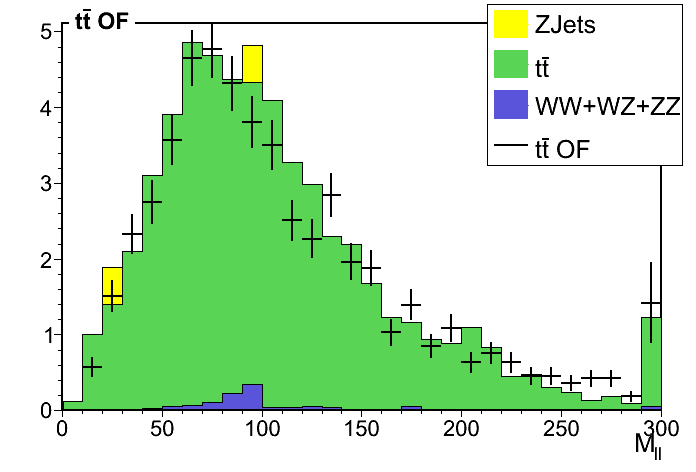
\includegraphics{plots/flavorsubdata.png}}
    \caption{Dilepton mass distribution for events passing the loose signal region selection. The solid histograms represent the yields in the same-flavor
      final state for each SM contribution, while the solid black line (OFOS) indicates the sum of the MC contributions in the opposite-flavor final state.
      %The observed ttbar yields inside the $Z$ mass window in the $ee$ and $\mu\mu$ final states are indicated. 
      The \ttbar distribution in the same-flavor final state is well-modeled by the OFOS prediction.}
    \label{fig:ttbar}
  \end{center}
\end{figure}

